\documentclass[10pt,a4paper]{ctexart}
\usepackage[margin=2.5cm]{geometry}
\usepackage[utf8]{inputenc}
\usepackage{amsmath}
\usepackage{amsfonts}
\usepackage{amssymb}
\usepackage{epsfig}
\usepackage{ifthen}
\usepackage{multicol}

%\newlength{\la}
%\newlength{\lb}
%\newlength{\lc}
%\newlength{\ld}
%\newlength{\lhalf}
%\newlength{\lquarter}
%\newlength{\lmax}
\newcommand{\xx}[4]{\\[.5pt]%
	\settowidth{\la}{A.~#1~~~}
	\settowidth{\lb}{B.~#2~~~}
	\settowidth{\lc}{C.~#3~~~}
	\settowidth{\ld}{D.~#4~~~}
	\ifthenelse{\lengthtest{\la > \lb}} {\setlength{\lmax}{\la}} {\setlength{\lmax}{\lb}}
	\ifthenelse{\lengthtest{\lmax < \lc}} {\setlength{\lmax}{\lc}} {}
	\ifthenelse{\lengthtest{\lmax < \ld}} {\setlength{\lmax}{\ld}} {}
	\setlength{\lhalf}{0.5\linewidth}
	\setlength{\lquarter}{0.25\linewidth}
	\ifthenelse{\lengthtest{\lmax > \lhalf}} {\noindent{}A.~#1 \\ B.~#2 \\ C.~#3 \\ D.~#4 } {
		\ifthenelse{\lengthtest{\lmax > \lquarter}} {\noindent\makebox[\lhalf][l]{A.~#1~~~}%
			\makebox[\lhalf][l]{B.~#2~~~}\par%
			\makebox[\lhalf][l]{C.~#3~~~}%
			\makebox[\lhalf][l]{D.~#4~~~}}%
		{\noindent\makebox[\lquarter][l]{A.~#1~~~}%
			\makebox[\lquarter][l]{B.~#2~~~}%
			\makebox[\lquarter][l]{C.~#3~~~}%
			\makebox[\lquarter][l]{D.~#4~~~}}}}
\newcommand{\xz}[1][1]{\nolinebreak\mbox{(\hspace{1cm})}\\\vspace{-0.33cm}}
\newcommand{\tk}[1][2.5]{\,\underline{\mbox{\hspace{#1 cm}}}\,}

\usepackage{setspace}

\usepackage{graphics}
\usepackage{float}
\usepackage{caption,subcaption}


\pagestyle{plain}
\title{\Large{\textbf{2022年全国高中数学联合竞赛一试A卷}}}
\date{2022年9月11日}
\author{制卷单位:江苏省数学学会}
%\author{学校\underline{\hspace{3cm}}姓名\underline{\hspace{3cm}} 城市\underline{\hspace{3cm}}}

\begin{document}
	\maketitle
	\subsection*{考生须知}
	\begin{enumerate}
		\item 答卷前,考生务必将自己的姓名和准考证号填写在答题卡上。
		\item 考试结束后,将本试卷和答题卡一并交回。
	\end{enumerate}
	请认真核对监考员在答题卡上所粘贴的条形码上的姓名、准考证号与您本人是否相符。	
	\subsection*{一、填空题,本大题共8小题,每小题8分,满分64分.}
	\begin{spacing}{1.8}
		\begin{itemize}
			\item[1.] 集合$A=\{A|n^3<2022<3^n,n\in Z\}$的所有元素之和为\tk.
			\item[2.] 设函数$f(x)=\frac{x^2+x+16}{x}(2\leq x\leq a)$,其中实数$a>2$,若$f(x)$的值域为$[9,11]$,则$a$的取值范围为\tk.
			\item[3.] 一枚不均匀的硬币,若随机抛掷它两次均得到正面的概率是均得到反面的概率的9倍,则随机抛掷它两次得到正面,反面各一次的概率为\tk. 
			\item[4.] 若复数$z$满足$\frac{z-3i}{z+i}$为负实数($i$为虚数单位),$\frac{z-3}{z+1}$为纯虚数,则$z$的值为\tk.
			\item[5.] 若四棱锥$P-ABCD$的棱$AB$,$BC$的长均为$\sqrt{2}$,其他各棱长均为1,则该四棱锥的体积为\tk.
			\item[6.]已知函数$y=f(x)$的图像既关于点$(1,1)$中心对称,又关于直线$x+y=0$轴对称,若$x\in (0,1)$时,$f(x)=\log_2{x+1}$,则$f(\log_2{10})$的值为\tk.
			\item[7.]在平面直角坐标系中,椭圆$\Omega$: $\frac{x^2}{4}+y^2=1$,$P$为$\Omega$上的动点,$A,B$为两个定点,其中$B$的坐标为$(0,3)$,若$\Delta ABC$的面积最小值为1,最大值为5,则线段AB的长为\tk.
			\item[8.]一个单位方格的四条边中,若有两条边染了颜色i,另两条边分别染了异于i色的另两种不同颜色,则称该单位方格是“i色主导”的.如图,一个1$\times$3方格表的表格线共含10条单位长线段,现要对这10条线段染色,每条线段染为红、黄、蓝三色之一,使得红色主导、黄色主导、蓝色主导的单位方格各有一个.这样的染色方式数为\tk(答案用数值表示).
			\begin{center}
				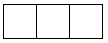
\includegraphics[width=0.2\textwidth]{tkt1.png}
			\end{center} 
		\end{itemize}
	\end{spacing}
	\newpage
	
	\subsection*{三、简答题, 本大题共3小题,满分56分.解答应写出文字说明、证明过程或演算步骤.}
	\begin{spacing}{1.8}
		\begin{itemize}
			\item[9.](本题满分16分)若$\Delta ABC$的内角$A,B,C$满足$\sin A=\cos B=\tan C$, 求$\cos ^3 A+\cos ^2 A-\cos A$的值.
			\item[10.](本题满分20分)给定正整数$(m,m\geq 3)$,设正项等差数列$\{a_n\}$与正项等比数列$\{b_n\}$满足:$\{a_n\}$的首项等于$\{b_n\}$的公比,$\{b_n\}$的首项等于$\{a_n\}$的公差,且$a_m=b_m$,求$a+m$的最小值,并确定当$a_m$取到最小值时$a_1$与$b_1$的公差.
			\item[11.](本题满分20分)在平面直角坐标系中,双曲线$\Gamma$: $\frac{x^2}{3}-y^2=1$对平面内不在$\Gamma$上的任意一点$P$,记$\Omega_P$为过点$P$且与$\Gamma$有两个交点的直线的全体.对任意直线$l\in \Omega_P$记,$MN$为$l$与$\Gamma$的两个交点,定义$f_p(l)=|PN|\cdot |PM|$,若存在一条直线$l_0\in \Omega_P$满足: $l_0$与$\Gamma $的两个交点位于$y$轴异侧,且对任意直线$l\in \Omega_P,l\neq l_0$, 均有$f_p(l)>f_p(l_0)$,则称$P$点为"好点",求所有好点所构成的区域的面积.
		\end{itemize}
	\end{spacing}
\end{document}